\begin{tikzpicture}[scale=0.8]
    % Definir los puntos
    \tkzDefPoint(0,0){A}
    \tkzDefPoint(-2,2){B}
    \tkzDefPoint(2,2){C}
    \tkzDefPoint(-2,-2){D}
    \tkzDefPoint(2,-2){E}

    % Dibujar las lineas y puntos
    \tkzDrawSegment[add=0 and 0.2,-Latex](A,B)
    \tkzDrawSegment[add=0 and 0.2,-Latex](A,C)
    \tkzDrawSegment[add=0 and 0.2,-Latex](A,D)
    \tkzDrawSegment[add=0 and 0.2,-Latex](A,E)
    
    \tkzDrawPoints(A,B,C,D,E)

    % Marcar los puntos
    \tkzLabelPoint[below left](B){$B$}
    \tkzLabelPoint[below right](C){$C$}
    \tkzLabelPoint[above right](E){$E$}
    \tkzLabelPoint[above left](D){$D$}
    \tkzLabelPoint[below](A){$A$}

    % Marcar los ángulos
    \tkzMarkAngle[arc=l,size=0.8,mark=|,color=red](B,A,D)
    \tkzMarkAngle[arc=l,size=0.8,mark=|,color=red](E,A,C)

    \tkzMarkAngle[arc=l,size=0.8,mark=||,color=blue](C,A,B)
    \tkzMarkAngle[arc=l,size=0.8,mark=||,color=blue](D,A,E)

\end{tikzpicture}